\documentclass[tikz,border=20pt]{standalone}
\usepackage[scaled=0.92]{helvet}
\renewcommand{\familydefault}{\sfdefault}
\usepackage[T1]{fontenc}
\usepackage{xcolor}

% Refined, distinct color palette for the three sets
\definecolor{colEspresso}{RGB}{185, 65, 30}   % Warm terracotta / espresso
\definecolor{colMilk}{RGB}{35, 130, 95}       % Fresh forest / sage green
\definecolor{colCold}{RGB}{30, 110, 185}      % Crisp ocean blue
\definecolor{darkText}{RGB}{30, 30, 35}
\definecolor{bgBox}{RGB}{249, 250, 251}
\definecolor{boxBorder}{RGB}{215, 220, 228}

\begin{document}
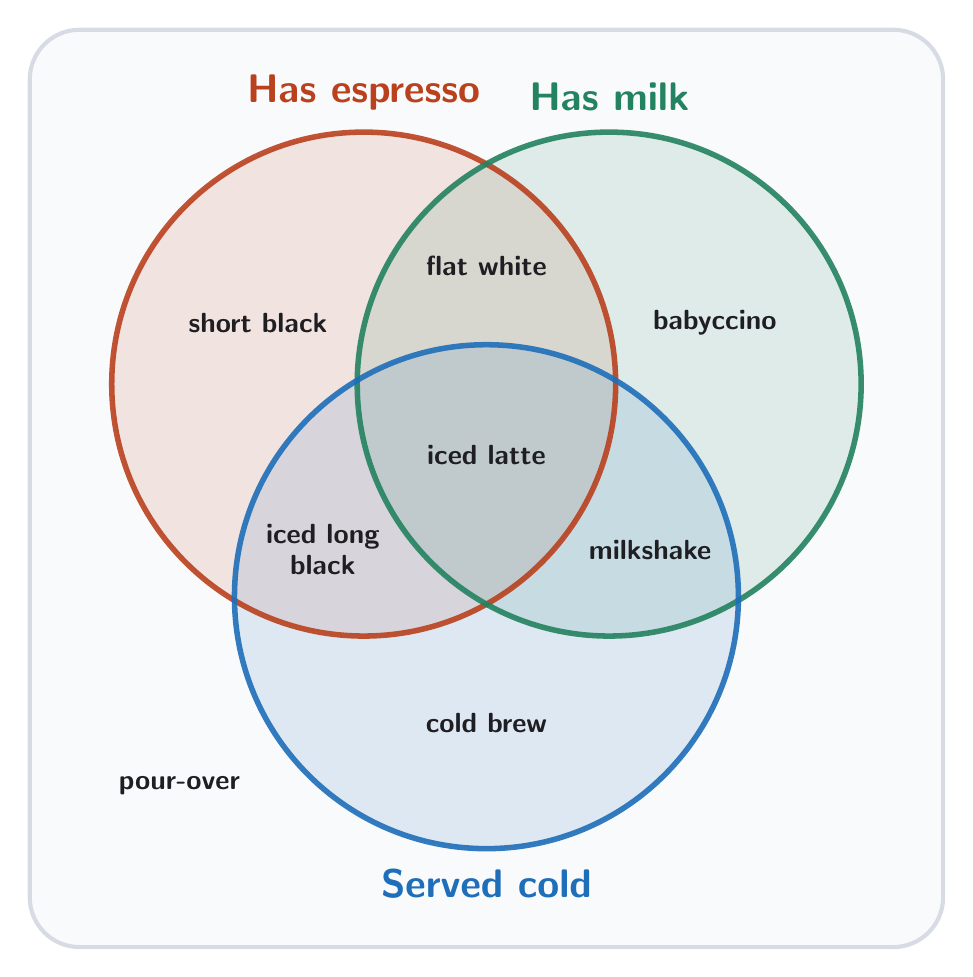
\begin{tikzpicture}[>=latex]

  % Universe / Bounding box (symmetric and balanced margins)
  \draw[rounded corners=18pt, fill=bgBox, draw=boxBorder, line width=1.5pt]
    (-5.8, -6.25) rectangle (5.8, 5.40);

  % Circles setup:
  % Centers at d=1.8, R=3.2
  % E: 150 deg (-1.5588,  0.900)
  % M:  30 deg ( 1.5588,  0.900)
  % C: 270 deg ( 0.0000, -1.800)
  \coordinate (cE) at (150:1.8);
  \coordinate (cM) at (30:1.8);
  \coordinate (cC) at (270:1.8);

  \def\R{3.2}

  % Filled circles with soft opacity for overlapping region distinction
  \begin{scope}[fill opacity=0.12]
    \fill[colEspresso] (cE) circle (\R);
    \fill[colMilk]     (cM) circle (\R);
    \fill[colCold]     (cC) circle (\R);
  \end{scope}

  % Circle outlines
  \draw[colEspresso, line width=2pt, draw opacity=0.9] (cE) circle (\R);
  \draw[colMilk,     line width=2pt, draw opacity=0.9] (cM) circle (\R);
  \draw[colCold,     line width=2pt, draw opacity=0.9] (cC) circle (\R);

  % Circle labels (Category names, centered over/under respective circle crests)
  \node[font=\bfseries\Large, text=colEspresso, anchor=south] at (-1.56, 4.25) {Has espresso};
  \node[font=\bfseries\Large, text=colMilk, anchor=south]     at ( 1.56, 4.25) {Has milk};
  \node[font=\bfseries\Large, text=colCold, anchor=north]     at ( 0.00, -5.15) {Served cold};

  % Helper style for drink nodes
  \tikzset{
    drink/.style={
      font=\bfseries\normalsize,
      text=darkText,
      align=center
    }
  }

  % --- 8 Drinks in their respective regions ---

  % 1. Has espresso ONLY: short black
  \node[drink] at (150:3.35) {short black};

  % 2. Has milk ONLY: babyccino
  \node[drink] at (30:3.35) {babyccino};

  % 3. Served cold ONLY: cold brew
  \node[drink] at (270:3.40) {cold brew};

  % 4. Has espresso + Has milk (not cold): flat white
  \node[drink] at (90:2.40) {flat white};

  % 5. Has espresso + Served cold (no milk): iced long black
  \node[drink] at (210:2.40) {iced long\\[-1pt]black};

  % 6. Has milk + Served cold (no espresso): milkshake
  \node[drink] at (330:2.40) {milkshake};

  % 7. Has espresso + Has milk + Served cold (all three): iced latte
  \node[drink] at (0, 0.0) {iced latte};

  % 8. Outside all three circles: pour-over
  \node[drink] at (-3.9, -4.2) {pour-over};

\end{tikzpicture}
\end{document}
